%%%%%%%%%%%%%%%%%%%%%%%%%%%%%%%%%%%%%%%%%%%%%%%%%%%%%%%%%%%%%%%%%%%%%%%%%%%%%%%%
% INTRODUCTION
\chapter{Introduction}
%%%%%%%%%%%%%%%%%%%%%%%%%%%%%%%%%%%%%%%%%%%%%%%%%%%%%%%%%%%%%%%%%%%%%%%%%%%%%%%%

File system metadata management is difficult to scale. The attention that the
topic has received, in both industry and academia, suggests that even
decoupling metadata IO from data IO so that these services can scale
independently~\cite{alam:pdsw2011-metadata-scaling, ghemawat:sosp2003-gfs,
hildebrand:msst2005-pnfs, weil:osdi2006-ceph, welch:fast2008-panasas,
xing:sc2009-skyfs} is insufficient for today's workloads. In the last 20 years,
many cutting-edge techniques for scaling file system metadata access, mainly
targeting POSIX IO's global and hierarchical semantics, have been proposed.

Unfortunately, techniques for scaling file system metadata access are
implemented in `clean-slate' file systems built from the ground up, so users
that want to leverage techniques from different file systems must provision
separate storage clusters. Adding software layers to the compute stack in this
way complicates system management because administrators must now (1) configure
data migrations across file system boundaries and (2) compare file system
metadata management techniques, which includes understanding implementations
and benchmarking systems with the workload.  Alternatively, developers can
integrate multiple techniques into an existing file system and expose
configuration parameters to let users select metadata management strategies.
While this lets users compare techniques and minimizes data movement, it
further increases the size of the stack because software layers are larger and
their internals are more complex.  This approach complicates system management
because if techniques do not match the workload or a new technique becomes
available, developers need to modify code, which takes time and jeopardizes the
robustness of the file system.

As a result of this complexity and perceived scalability limitation,
communities are abandoning global namespaces.  Our fundamental insight is that
many file systems have similar internals and that the policies from
cutting-edge techniques for file system metadata access can be expressed in a
system-agnostic way. So application developers can design policies based on
their knowledge of the application, without having to understand storage system
internals.  While separating policy from mechanism is not a new
idea~\cite{mckusick:fast2015-FFS}, we show that given the right interfaces,
application developers can guide file system metadata management techniques
using domain-specific knowledge.  To that end, we use the programmable storage
approach~\cite{sevilla:eurosys17-malacology} to embed policy engines into file
system metadata substrates to control the behavior, performance, and
transparency of the entire software stack.

\section{Contributions}

Using the programmable storage approach, we design policies for three metadata
management techniques: subtree load balancing, subtree semantics, and subtree
schemas.  The first two expand on a strong foundation of related work while the
third is a novel idea. 

First, we present a methodology for programmable load balancing policies for
file system metadata.  To help decouple policy from mechanism, we introduce a
programmable storage system, Mantle, that lets the designer inject custom
balancing logic. We show the flexibility and transparency of this approach by
replicating the strategy of a state-of-the-art metadata balancer and conclude
by comparing this strategy to other custom balancers on the same system. We
also show how the data management language and policy engine from Mantle turns
out to be an effective control plane for managing ZLog sequencers and ParSplice
caches.

Second, we present a methodology for programmable consistency and durability in
a global namespace. Our prototype, Cudele, lets clients specify their
consistency/durability requirements and dynamically assign them to subtrees in
the same namespace, allowing users to optimize subtrees over time and space for
different workloads. We confirm the performance benefits of techniques
presented in related work but also explore new consistency/durability metadata
designs, all integrated over the same storage system. By custom fitting a
subtree to a create-heavy application, we we show performance improvements when
we custom fit subtree semantics to applications such as checkpoint-restart
(91.7\(\times\) speedup), user home directories (0.03 standard deviation from
optimal), and users checking for partial results (2\% overhead).

Third, we present a methodology for generating namespaces automatically and
lazily, without incurring the costs of traditional metadata management,
transfer, and materialization.  We introduce namespace generators and schemas
to describe file system metadata structure in a compact way. If clients and
servers can express the namespace in this way, they can compact metadata,
modify large namespaces more quickly, and generate only relevant parts of the
namespace. The result is less network traffic, storage footprints, and overall
metadata operations.  Our prototype, Tintenfisch, is a programmable file system
that enables namespace generators.

These contributions have mostly been prototyped on Ceph. Mantle was merged into
Ceph and funded by the Center for Research in Open Source Software and Los
Alamos National Laboratory. Malacology and Mantle were featured in the Next
Platform magazine and the 2017 Lua Workshop. Finally, Malacology and Cudele are
the first Popper-compliant conference papers.

\section{Outline}

\begin{figure}[tb]
  \centering
  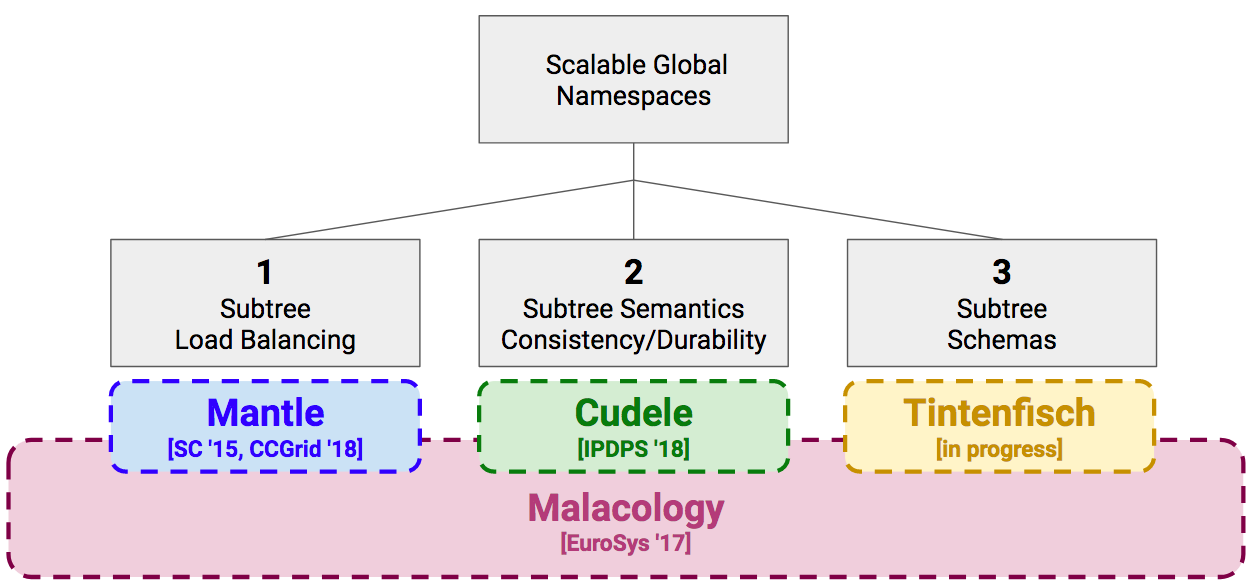
\includegraphics[width=1\textwidth]{./chapters/overview.png}
  \caption{An outline of this thesis.}
  \label{fig:thesis-overview}
\end{figure}

An outline of the thesis is shown in Figure~\ref{fig:thesis-overview}.

Chapter~\ref{chp:related-work} discusses the file system metadata management
problem and shows why today's jobs impose these types of workloads. We also
survey related work for providing scalability while enforcing POSIX IO
semantics. Chapter~\ref{chp:prototyping-platform} describes our prototyping
platform, Ceph, and the interfaces we added to create a programmable storage
system called Malacology.

Chapter~\ref{chp:mantle} describes the Mantle environment and API for load
balancing subtrees across a metadata cluster. We motivate the framework by
measuring the advantages of file system workload locality and examining the
current CephFS implementation designed in~\cite{weil:osdi2006-ceph,
weil:sc2004-dyn-metadata}. We show that the framework can replicate techniques
from related work and show load balancers that work well for different
workloads. Chapter~\ref{chp:mantle-beyond} shows the generality of the approach
by using the Mantle API for load balancing in ZLog, an implementation of the
CORFU~\cite{balakrishnan_corfu_2012} API on Ceph, and for cache management in
ParSplice~\cite{perez:jctc20150parsplice}, a molecular dynamics simulation
developed at Los Alamos National Laboratory.

Chapter~\ref{chp:cudele} describes the Cudele API and framework for relaxing
consistency and durability semantics in a global file system namespace. We
focus on the building blocks called mechanisms and show how administrators can
build application-specific subtrees.  We motivate Cudele by measuring the POSIX
IO overheads using CephFS and by examining current workloads in HPC and
Hadoop/Spark. The microbenchmarks show the performance of individual mechanisms
while the macrobenchmarks model real-world use cases.

Chapter~\ref{chp:tintenfisch} describes Tintenfisch, which lets clients and
servers generate subtrees to reduce network traffic, storage footprints, and
file system metadata load. We examine three motivating examples from three
different domains: high performance computing, high energy physics, and large
scale simulations. We then present namespace schemas for categorizing file
system metadata structure and namespace generators for compacting metadata.

Chapter~\ref{chp:conclusion} concludes and outlines future work.

